%%%%%%%%%%%%%%%%%%%%%%%%%%%%%%%%%%%%%%%%%%%%%%%%%%%%%%%%%%%%%%%%%%%%%%%%%%%%%%%
%  GPW-26 Extended Abstract (A4, 2ページ以内, 10pt以上)
%
%  ★ コンパイル: LuaLaTeX (luatexja) ★
%    Overleaf: Compiler を「LuaLaTeX」に設定するだけ (latexmkrc 不要)
%    ローカル/VSCode: latexmk (gpw_paper/latexmkrc が lualatex を指定)
%
%  図: elo_final_zero.pdf / asahi_L1H2.pdf / asahi_L2H2.pdf /
%      asahi_IG_policy.pdf / asahi_IG_value.pdf / arch 図
%%%%%%%%%%%%%%%%%%%%%%%%%%%%%%%%%%%%%%%%%%%%%%%%%%%%%%%%%%%%%%%%%%%%%%%%%%%%%%%
\documentclass[a4paper,10pt,twocolumn]{ltjsarticle}

\usepackage{graphicx}
\usepackage[table]{xcolor}
\usepackage[margin=16mm]{geometry}
\linespread{0.97}
\usepackage{amsmath}
\usepackage{tikz}
\usetikzlibrary{positioning,arrows.meta,calc}
\usepackage{titlesec}
% 見出し前後の余白を詰めて2ページに収める
\titlespacing*{\section}{0pt}{3pt plus 1pt}{2pt}
\titlespacing*{\subsection}{0pt}{2pt plus 1pt}{1pt}
\setlength{\parindent}{1\zw}
\pagestyle{empty}

% 図と本文・キャプションの余白を詰める
\setlength{\textfloatsep}{2pt plus 1pt minus 1pt}   % 段上下の float と本文の間
\setlength{\intextsep}{4pt plus 1pt minus 1pt}      % 本文中 float の上下
\setlength{\floatsep}{4pt plus 1pt minus 1pt}       % float 同士の間
\setlength{\abovecaptionskip}{2pt}                  % 図とキャプションの間
\setlength{\belowcaptionskip}{1pt}

% RRTRRT の色付きブロック
\newcommand{\rblk}{\colorbox{blue!15}{\makebox[2.6ex]{R}}}
\newcommand{\tblk}{\colorbox{orange!35}{\makebox[2.6ex]{T}}}

% 所属をマーカ無し脚注として第1段下部に出す（IPSJ形式）
\newcommand{\blfootnote}[1]{%
  \begingroup
  \renewcommand\thefootnote{}\footnote{#1}%
  \addtocounter{footnote}{-1}%
  \endgroup}

% 画像があれば挿入,無ければ枠(どちらでもコンパイル可)
\newcommand{\figorbox}[3]{%
  \IfFileExists{#1}{\includegraphics[width=\linewidth]{#1}}%
  {\fbox{\parbox[c][#2][c]{0.9\linewidth}{\centering\scriptsize #3}}}}

\begin{document}

\twocolumn[{%
\vspace{-9mm}
\begin{center}
  {\LARGE\bfseries ResTNet による将棋 AI の解釈:\\[2pt]
   Transformer のAttention機構による着目領域の可視化と妥当性の検証}\\[4pt]
  {\large Interpreting a Shogi AI Built on ResTNet:\\
   Visualizing and Validating Attention over the Board}\\[5pt]
  {\large 横山 凜\textsuperscript{1,a)}\qquad
   Wei Ting-Han\textsuperscript{1,b)}}\\[4pt]
\end{center}
}]

\blfootnote{\noindent
1\quad 高知工科大学\\
\phantom{1\quad}Kochi University of Technology, Kami, Kochi 782--8502, Japan\\
a)\quad 305151a@gs.kochi-tech.ac.jp\quad
b)\quad tinghan.wei@kochi-tech.ac.jp}

%============================================================================
\section{はじめに}
AlphaZero 等の深層強化学習に基づく AI は超人的な性能を達成した
一方，判断の理由を人間が読み取りにくい．この不透明性は医療診断や自動運転など
説明が求められる分野で障壁となるため，判断根拠を説明する解釈性（説明可能 AI，
XAI）の研究には価値がある．

XAI 手法の検証にはゲームが適する．定石・手筋という言語化された知識と照合でき，
再現も容易だからである．中でも将棋は，囲碁・Hex・オセロに比べ持ち駒・成り・
非対称な利き（駒が動ける方向・範囲）など駒の扱いが多様で行動空間が格段に大きく，特徴量・選択肢が膨大な
実世界モデルへの応用可能性を示す検証対象として適している．

本研究では，Residual ブロック（R）と Transformer ブロック（T）を
交互配置し局所（近くのマス同士）と大局（盤面全体）の知識を扱う ResTNet~\cite{restnet} を対象とする．先行研究は囲碁等で
Attentionが長距離パターンを捉えると示したが，将棋への適用例は無い．そこで ResTNet を
将棋に初適用して自己対戦学習を行い，着目領域を可視化してその妥当性を将棋の
言葉で検証する．

%============================================================================
\section{手法}
\subsection{ResTNet と自己対戦学習}
入力は MiniZero の将棋表現に従う $362$ チャネルの $9\times9$
テンソル（各駒種の配置・持ち駒・手番・経過手数などを $362$ 枚の平面で表したもの）
であり，出力は
全合法手に対応する policy と局面の value である．ネットワークは R ブロックと T ブロックを
RRTRRT の順に 6 段重ね，隠れチャネル 256 とした（図~\ref{fig:arch}）．R は
畳み込みで近くのマスにある駒の利きを，T は self-attention で盤面全体の関係を捉える．学習は Gumbel
AlphaZero（シミュレーション 64，サンプル 16）を用い，1 反復あたり
自己対戦 2000 局・最適化 200 ステップとして計 300 反復（自己対戦約 60 万局）を
単一 GPU で行った．

\begin{figure}[htbp]
  \centering
  \fbox{%
  \begin{tikzpicture}[
      font=\scriptsize,>=Stealth,
      blk/.style={draw, rounded corners=1.5pt, minimum height=7mm, minimum width=6mm,
                  inner sep=1pt, font=\bfseries},
      R/.style={blk, fill=blue!15, draw=blue!55},
      T/.style={blk, fill=orange!35, draw=red!80, line width=1pt},
      io/.style={align=center},
    ]
    \node[io] (in) {入力\\[-2pt]{\tiny 362ch,\,$9{\times}9$}};
    \node[R, right=2.6mm of in] (r1) {R};
    \node[R, right=1.6mm of r1] (r2) {R};
    \node[T, right=1.6mm of r2] (t1) {T};
    \node[R, right=1.6mm of t1] (r3) {R};
    \node[R, right=1.6mm of r3] (r4) {R};
    \node[T, right=1.6mm of r4] (t2) {T};
    \node[io, right=2.6mm of t2] (out) {Policy\\[-2pt]/\,Value};
    \draw[->] (in) -- (r1);
    \draw[->] (r1) -- (r2); \draw[->] (r2) -- (t1); \draw[->] (t1) -- (r3);
    \draw[->] (r3) -- (r4); \draw[->] (r4) -- (t2);
    \draw[->] (t2) -- (out);
    % T ブロック（可視化対象）を強調: 両 T から下向き矢印＋注記
    \coordinate (lab) at ($(t1)!0.5!(t2) + (0,-6mm)$);
    \draw[red!80,->] (t1.south) -- (t1.south|-lab);
    \draw[red!80,->] (t2.south) -- (t2.south|-lab);
    \node[red!70!black, font=\tiny, below=4.5mm of {$(t1)!0.5!(t2)$}]
      {T の Attention を可視化};
  \end{tikzpicture}}\\[3pt]
  {\scriptsize \colorbox{blue!15}{\,R\,}\,= Residual（畳み込み；近くの駒の利き）\quad
   \colorbox{orange!35}{\,T\,}\,= Transformer（self-attention；盤面全体）}
  \caption{ResTNet の構成（RRTRRT）．Residual ブロック（R，青）と Transformer ブロック
    （T，橙）を交互に 6 段配置し，隠れチャネル 256．可視化対象は T ブロックの
    attention weight である．}
  \label{fig:arch}
\end{figure}

\subsection{解釈手法}
主たる解釈手法として Attention Map を用いる．T ブロックの self-attention は，盤面の
各マスを一つの単位（トークン）として扱い，マスとマスの関連の強さ（attention
weight）を行列で与える．そこで，着目したい手のマス，すなわち盤上を動く手なら移動元，
駒打ちなら打つ先を起点（クエリ）とし，そこから全 81 マスへの attention weight を
取り出して，$9\times9$ の盤面上に
ヒートマップとして重ねる．各マップは最大のマスを 1・最小を 0 とする min-max 正規化で
示す．元の attention weight は 81 マスの合計が 1 だが，正規化後の値は相対的な強さを表す．
AttentionはHeadごとに役割が異なりうるため，特定のLayer・
Headを指定して個別に可視化し，得られた着目領域を将棋の形勢判断・手筋と照合する．

補助的に Integrated Gradients (IG) を併用する．IG は，入力の各マスが出力に
どれだけ効いているかを勾配から調べる手法であり，これを最善手の policy 出力・
value 出力に適用する．Attention（モデルがどこを見るか）と IG（出力がどのマスに
敏感か）は観点が異なり，両者を合わせて着目の妥当性を確かめる．

%============================================================================
\section{結果と考察}
\subsection{学習の進行}
学習各段階のモデル同士を総当たりで対戦させ，相対 Elo を Bradley--Terry モデル
（MM 法）で算出した（図~\ref{fig:elo}）．最弱（初期）モデルを 0 とした相対 Elo は
反復を通じてほぼ単調に増加し，最終モデル（自己対戦約 60 万局）で約 $2670$ Elo に
達した．学習段階の逆転はほとんど無く，引き分け率も低い．これは ResTNet が将棋でも
自己対戦学習で一貫して棋力を向上させることを示す．なお本 Elo は学習過程のモデル間で
比べた相対的な値である．

\begin{figure}[htbp]
  \centering
  \figorbox{elo_final_zero.pdf}{32mm}{elo\_final\_zero.pdf}
  \caption{学習ステップに対する自己対局 Elo（最弱モデルを 0 基準）．
    ほぼ単調に増加し，最終モデルで約 2670 Elo に達する．}
  \label{fig:elo}
\end{figure}

\subsection{Attentionの可視化と妥当性}
学習済み最終モデルに，藤井--羽生戦（2018 年朝日杯）118 手目の寄せ（終盤の攻め）
局面（先手番）を入力した．実戦ではこの局面で先手が▲4七桂打を着手し，直後に後手が
投了している．この着手マス 4七をクエリとした Attention Map を図~\ref{fig:attn}
に示す．Layer が深まるにつれ着目の粒度が変化する様子がみられた．

浅いLayer（L1H2，図~\ref{fig:attn}(a)）ではAttentionが盤面全体にほぼ均等に分散し，
少数マスへの偏りを表す集中度は 0.2\% と低く，特定マスへの強い着目は現れない．一方，
深いLayer（L2H2，
図~\ref{fig:attn}(b)）ではより集中的になり（集中度 5.4\%），先手の攻めの拠点である
7七のと金へ最も強くAttentionが向き，次いで敵玉（5五）とその周辺を参照する．
すなわち，深いLayerほど攻め駒と敵玉という寄せの要点へ着目が移る傾向がみられる．

もっとも本局面は終盤の混戦であり，Attentionは全体としてやや散漫である．寄せの主眼が
攻め駒（7七）と敵玉（5五）に置かれる点は将棋的に妥当だが，浅いLayerの分散度の
高さも含め，弱いモデルにおける着目の限界を示す例でもある．

\begin{figure}[htbp]
  \centering
  \begin{minipage}[t]{0.49\linewidth}\centering
    \IfFileExists{asahi_L1H2.pdf}{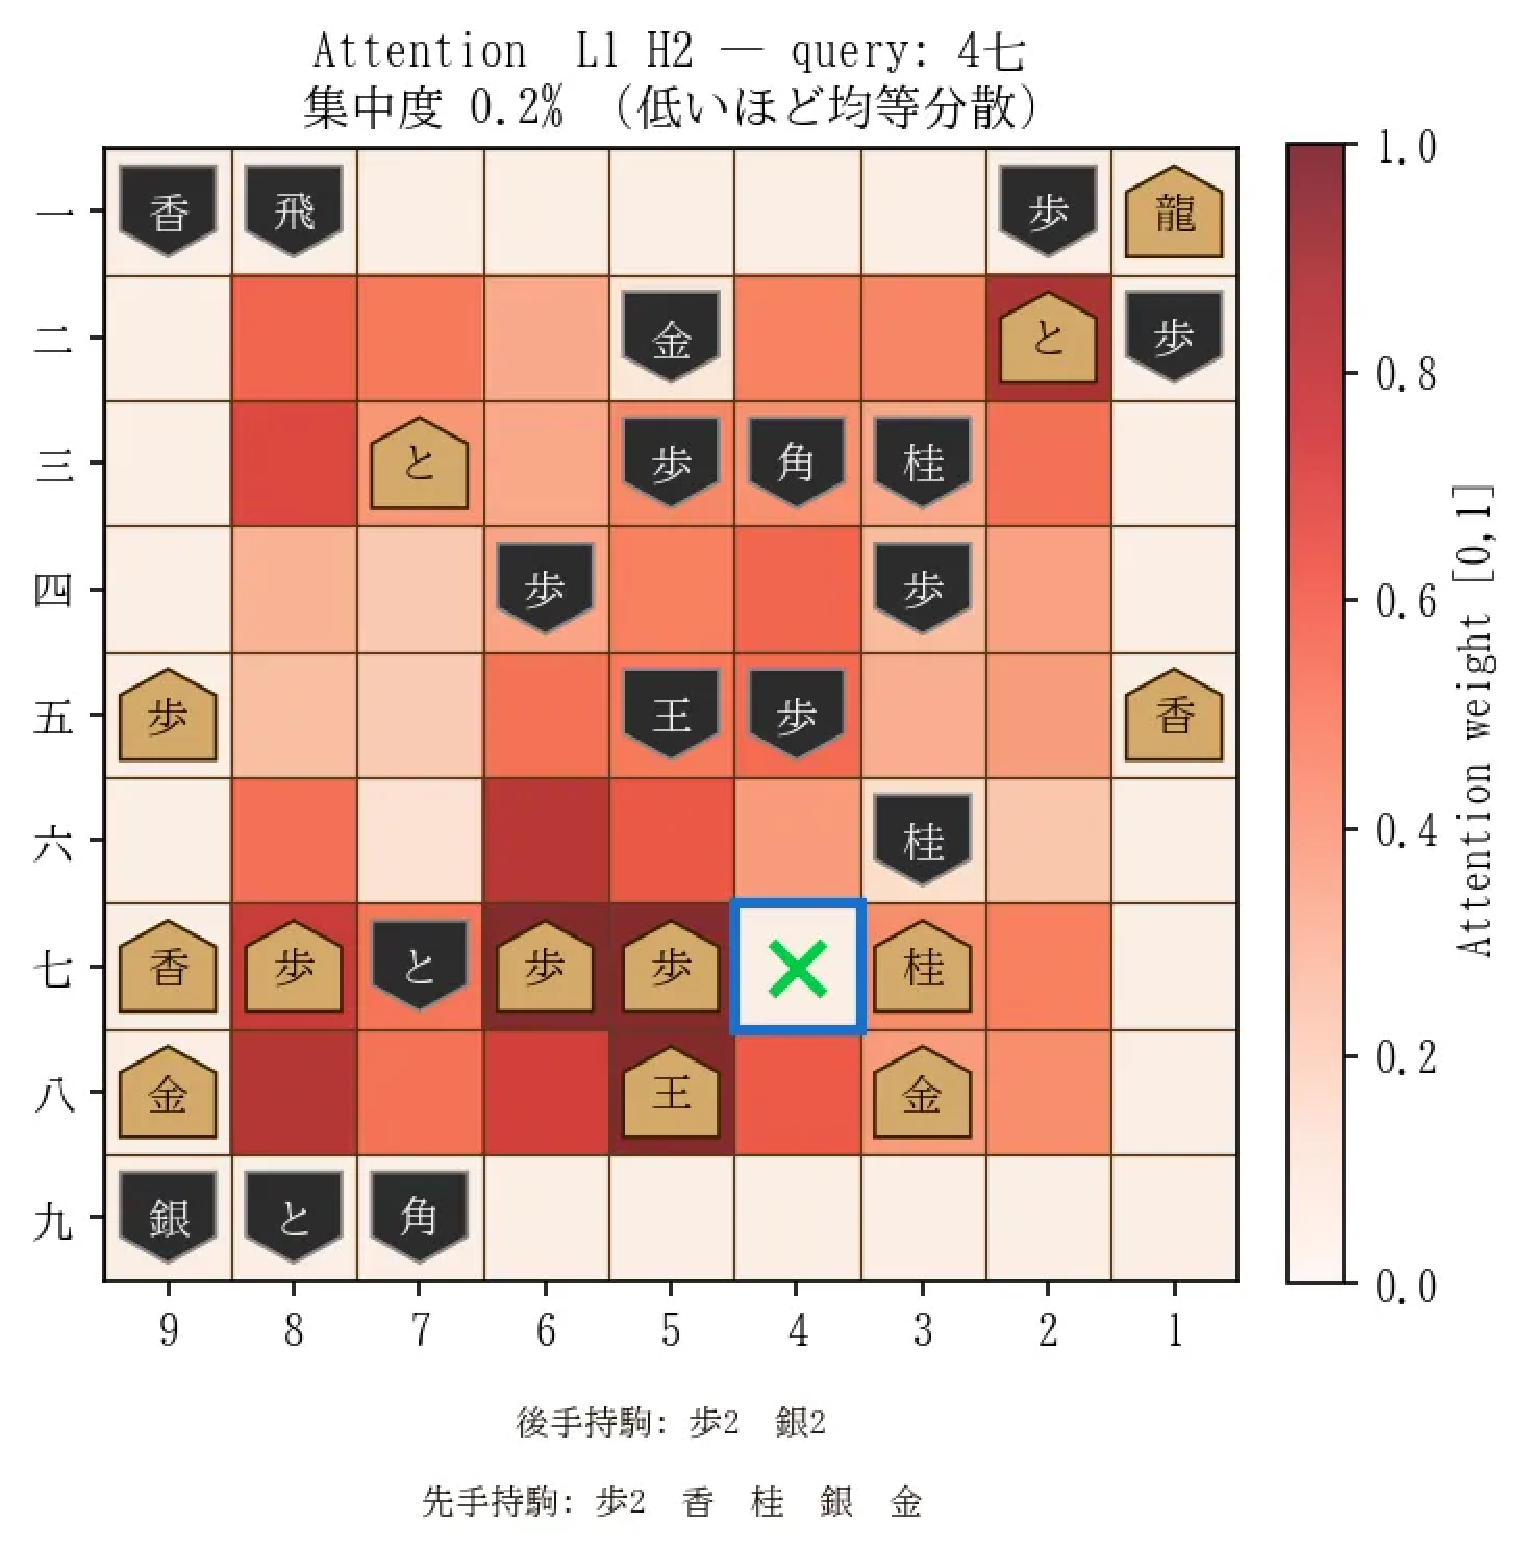
\includegraphics[width=\linewidth]{asahi_L1H2.pdf}}%
      {\fbox{\parbox[c][26mm][c]{0.9\linewidth}{\centering\scriptsize L1H2}}}\\[1pt]
    {\scriptsize (a) L1H2}
  \end{minipage}\hfill
  \begin{minipage}[t]{0.49\linewidth}\centering
    \IfFileExists{asahi_L2H2.pdf}{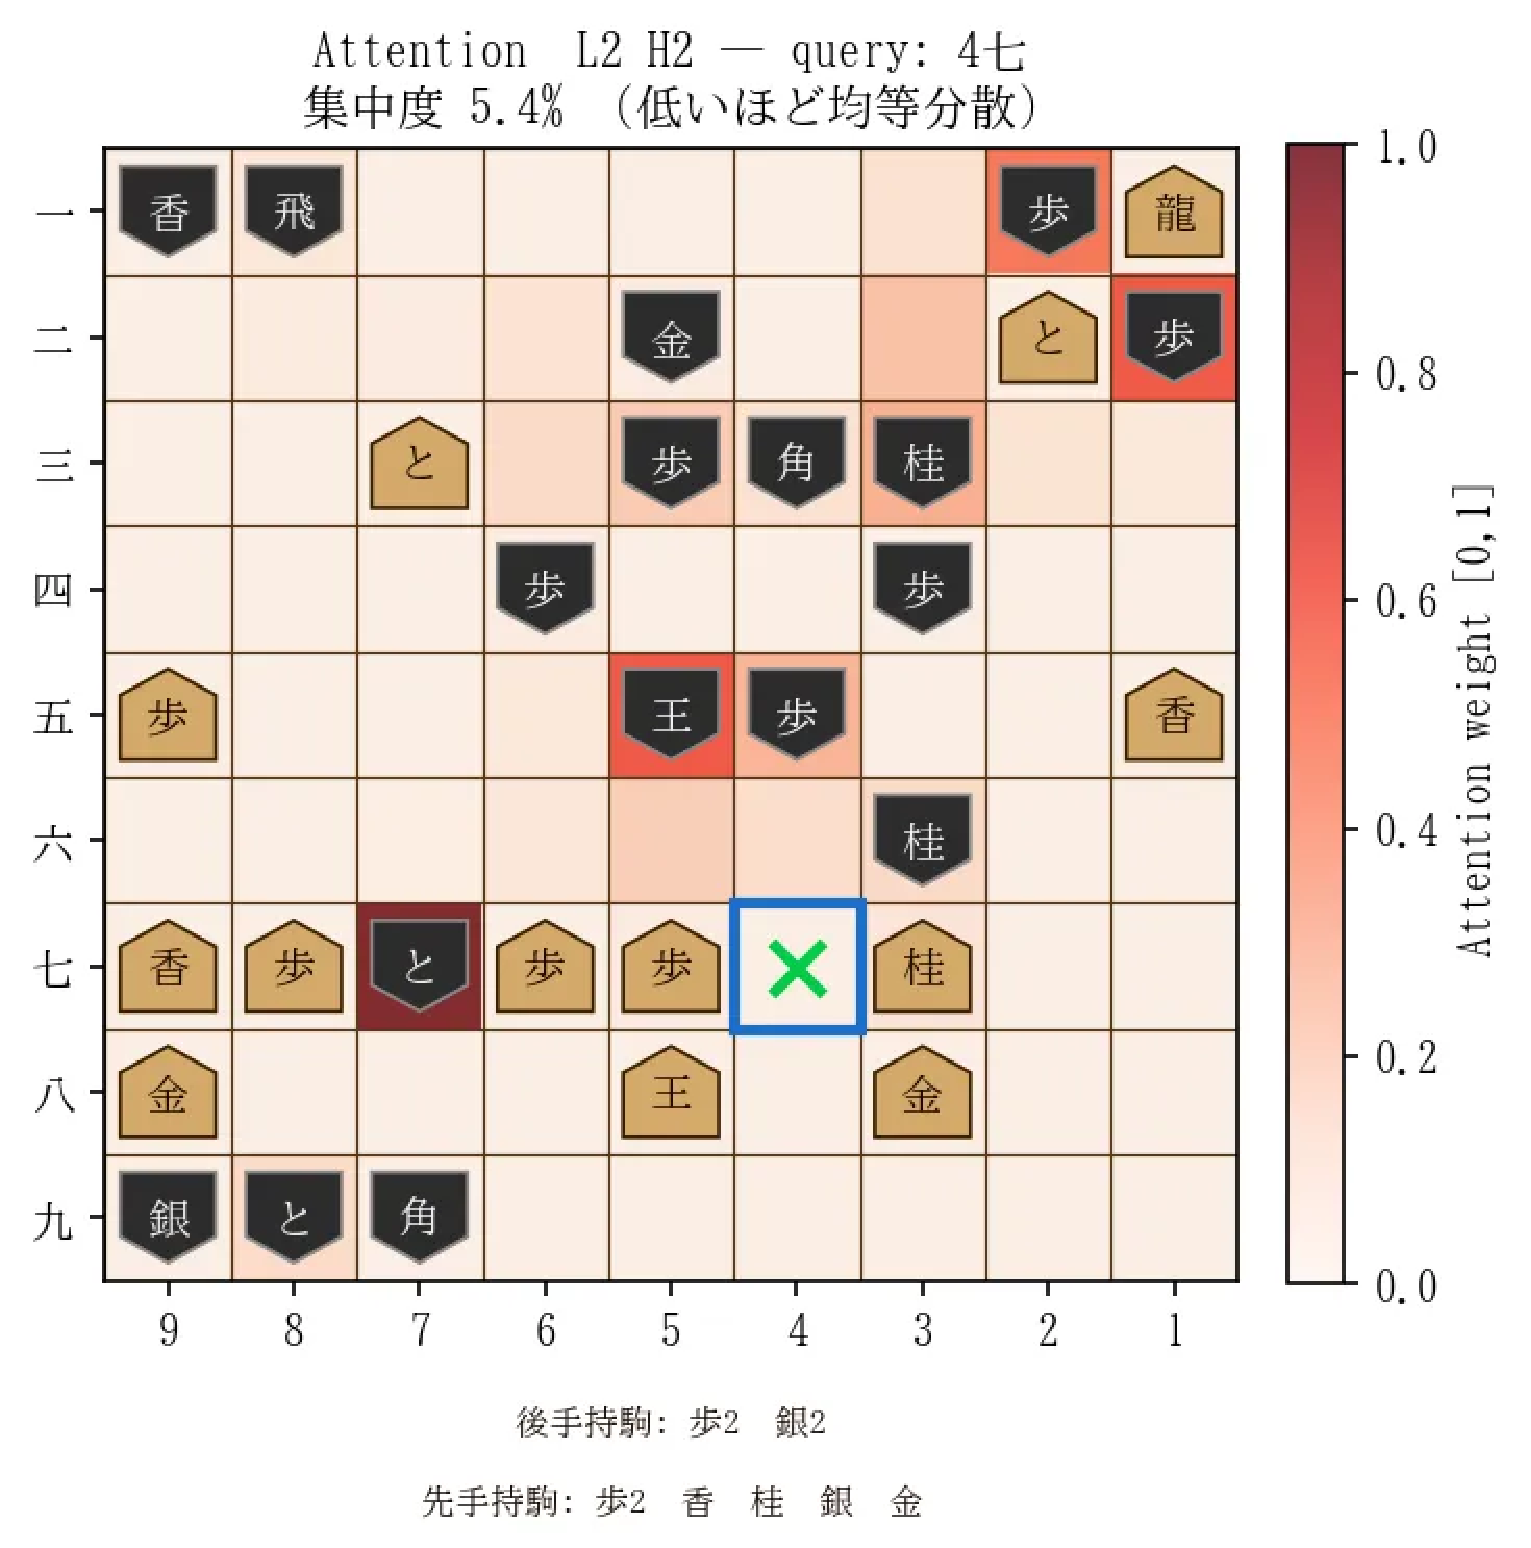
\includegraphics[width=\linewidth]{asahi_L2H2.pdf}}%
      {\fbox{\parbox[c][26mm][c]{0.9\linewidth}{\centering\scriptsize L2H2}}}\\[1pt]
    {\scriptsize (b) L2H2}
  \end{minipage}
  \caption{藤井--羽生戦 118 手目（先手番，着手▲4七桂打）の Attention Map．
    クエリは 4七．(a) 浅いLayer は全体に分散（集中度 0.2\%），
    (b) 深いLayer は攻めの拠点 7七のと金と敵玉 5五へ集中（集中度 5.4\%）し，
    Layer 間で着目の粒度が異なる．}
  \label{fig:attn}
\end{figure}

\subsection{IG との対応}
同一局面に対し，policy（着手▲4七桂打）および value の出力へ IG を適用した結果を
図~\ref{fig:ig} に示す．policy への IG は先手玉周辺と先手の攻め・守り駒に，value への
IG は敵の攻め駒と先手玉に大きな寄与を示し，いずれも先手玉周辺へ反応が集まる．終盤
における玉の安全重視という点で Attention Map と整合し，
観点の異なる二手法が同様の領域を指すことは，可視化された着目の妥当性を補強する．

\begin{figure}[htbp]
  \centering
  \begin{minipage}[t]{0.49\linewidth}\centering
    \IfFileExists{asahi_IG_policy.pdf}{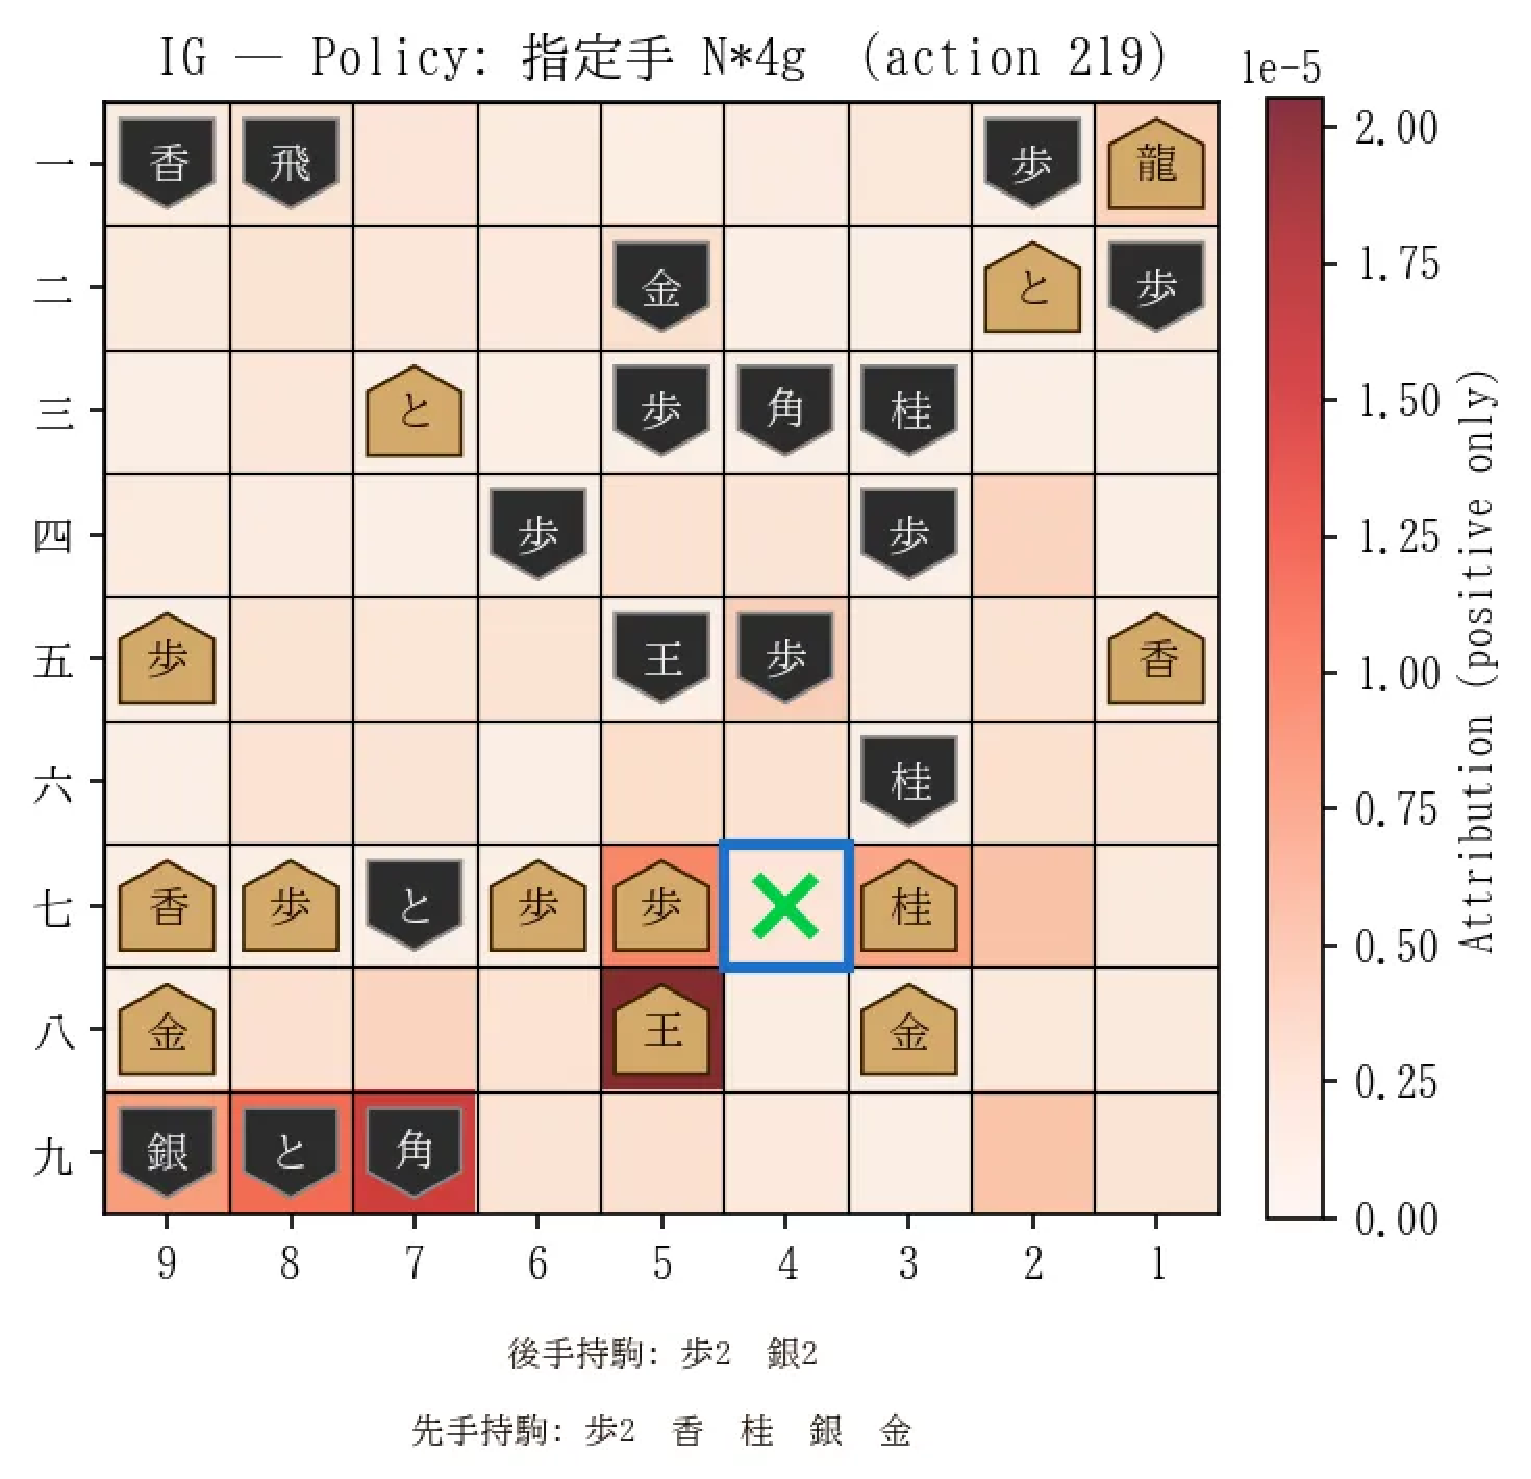
\includegraphics[width=\linewidth]{asahi_IG_policy.pdf}}%
      {\fbox{\parbox[c][26mm][c]{0.9\linewidth}{\centering\scriptsize IG policy}}}\\[1pt]
    {\scriptsize (a) policy への IG}
  \end{minipage}\hfill
  \begin{minipage}[t]{0.49\linewidth}\centering
    \IfFileExists{asahi_IG_value.pdf}{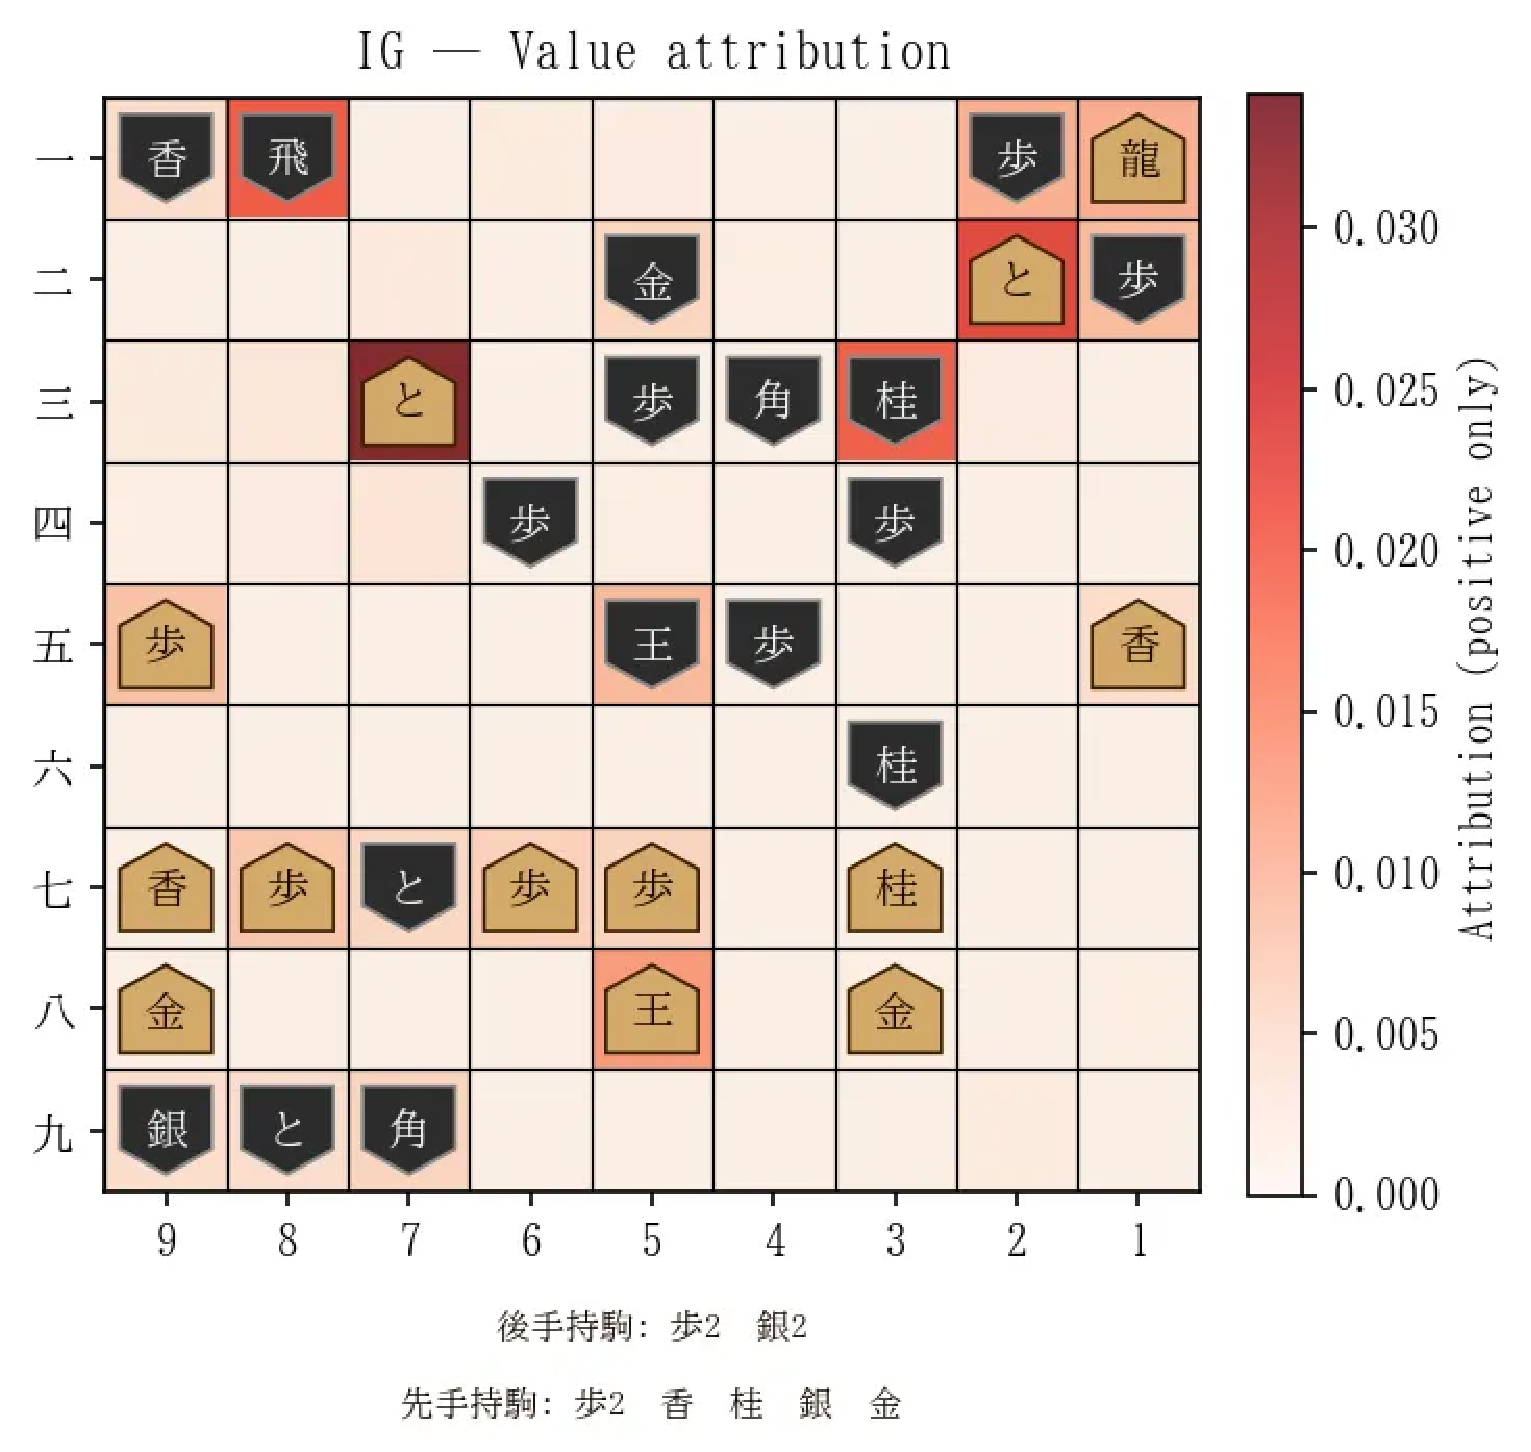
\includegraphics[width=\linewidth]{asahi_IG_value.pdf}}%
      {\fbox{\parbox[c][26mm][c]{0.9\linewidth}{\centering\scriptsize IG value}}}\\[1pt]
    {\scriptsize (b) value への IG}
  \end{minipage}
  \caption{policy（着手▲4七桂打）および value への IG の各マス寄与．
    (a) は先手玉（5八）周辺と攻め駒（7九角・3七桂・5七歩），
    (b) は敵の攻め駒（7三と・8一飛・3三桂）と先手玉に寄与が大きく，
    Attention Map と整合する．}
  \label{fig:ig}
\end{figure}

\subsection{考察}
本モデルのAttentionは特定のマスに強く集中せず盤面全体に散らばる傾向があり，これは
学習量が控えめ（約 60 万局）なためと考えられる．それでもHeadごとに見ると，
将棋的に妥当なマスへAttentionが向いており，解釈手法が将棋でも有効に働くことを示す．

一方で本手法には現時点で限界がある．入力は $9\times9$ の平面を 362 枚重ねた特徴量
として与えられるが，持ち駒は盤上の特定マスに存在しない情報（駒種ごとの枚数）で
ある．この非空間的な情報を平面表現に含めるため，現状の設計では各枚数を盤面全体へ
一様に敷いた定数平面として符号化している．その結果，持ち駒チャネルは全マスに同じ
値で乗ってマス間の差を生まず，対応するトークンを持たない．マス対マスの関係量である
単純な Attention Map からは，このように一様分布させた持ち駒の特徴が盤上のどこにどう
効くかを直接読み取ることは難しい．もっとも，持ち駒を除いた入力との Attention の差分
を取るなど，Attention の枠内でも手がかりを得られる可能性は残されており，どこまで
捉えられるかは今後の検証課題である．持ち駒の寄与をどのように可視化・評価するかは，
複数のアプローチを比較しながら論文本体投稿までに検討する．

%============================================================================
\section{おわりに}
ResTNet を将棋に初適用し，自己対戦学習により自己対局 Elo で測った棋力がほぼ単調に
向上することを確認した．また Attention Map と IG により，学習済みモデルが深いLayer
で攻め駒や玉の安全といった寄せの要点に対応するマスへ着目する様子を可視化した．ただし
本モデルのAttentionは全体として散漫であり，この対応が他局面でも一般に成り立つかは
単一局面のみからは判断できない．今後は，多数の局面や他のネットワーク構成での検証，
より大規模な学習，外部エンジンとの対局による棋力評価を進める．

%============================================================================
\begin{thebibliography}{9}
\small
\bibitem{restnet} Ju, Y.-R.\ et al.: Bridging Local and Global Knowledge via
  Transformer in Board Games, \textit{Proc.\ IJCAI} (2025).
\end{thebibliography}

\end{document}
